\documentclass[a4paper,12pt]{article}

\usepackage[a4paper]{geometry}
\geometry{margin={1cm,1.2cm}}
\usepackage[francais]{babel}


\usepackage{multicol}
%\usepackage{nopageno} %pas de numérotation de page
\pagestyle{plain} %numérotation en bas de page, pas d'entête
\usepackage{hyperref}
%\usepackage[latin1]{inputenc}


%%%%%%%%%%%%%%%%%%%%%%%%%%%%%%%%%%%%%%%%%%%%%%%%%%%%%%%%%%%%%%%%%%%%%%%%%%%%%%%%%%%%%

\usepackage[utf8]{inputenc} 
\usepackage{amssymb,amsmath}
\usepackage{stmaryrd}
\usepackage{amsthm}
\usepackage{amscd}
%\usepackage{mathrsfs}
%\usepackage{amsfonts}
%\usepackage[T1]{fontenc}
%\usepackage{theorem}
\usepackage{lscape}
\usepackage{variations}  % pour faire des tableaux de variations
\usepackage{dsfont}
\usepackage{fancyvrb} % pour mettre Verbatim dans une box
\usepackage{moreverb} % pour mettre Verbatim dans une box 
\usepackage{comment} % pour afficher ou non les commentaires, solutions
%\usepackage{slashbox} % pour dans un tabular, couper une case en deux
\usepackage{boxedminipage} % pour cadrer du texte
\usepackage{listings}

% Pour les figures
\usepackage{subfig}
\usepackage{calc} % Pour pouvoir donner des formules dans les d�finitions de longueur
\usepackage{graphicx} % Pour inclure des graphiques 
% Attention : pour inclure des .jpg comme dans l'exemple (ou des .png ou .pdf)
% il faut compiler directement en pdf (commande pdflatex).
% Pour inclure des .eps, il faut compiler avec latex + dvips + ps2pdf.
\usepackage{psfrag}
\usepackage{color}

%%%%%%%%%%%%%%%%%%%%%%%%%%%%%%%%%%%%%%%%%%%%%%%%%%%%%%%%%%%%%%%%%%%%%%%%%%%%%%%%%%%%%

\theoremstyle{definition}
\newtheorem{thm}{Théorème}
%\theorembodyfont{\rmfamily}
\newtheorem*{defn}{Définition}
\newtheorem{exercice}{Exercice}
\newtheorem*{problem}{Problème}
\newtheorem{prop}{Proposition}
\newtheorem{corollaire}{Corollaire}
\newtheorem*{lemme}{Lemme}
\newtheorem*{remark}{Remarque}
\newtheorem*{notation}{Notation}
\newtheorem*{ex}{Exemple}
\newtheorem*{ppe}{Propriété}
\newtheorem*{meth}{Méthode}
\newtheorem*{rappel}{Rappel}
\newtheorem*{voca}{Vocabulaire}
\newtheorem*{solution}{Solution}   

\setlength{\columnseprule}{0.5pt}


%%%%%%%%%%%%%%%%%%%%%%%%%%%%%%%%%%%%%%%%%%%%%%%%%%%%%%%%%%%%%%%%%%%%%%%%%%%%%%%%%%%%%

\newcommand{\bi}{\bigskip}
\newcommand{\dsp}{\displaystyle}
\newcommand{\noi}{\noindent}
\newcommand{\ov}{\overline}
\newcommand{\dsum}{\displaystyle \sum}
\newcommand{\dprod}{\displaystyle \prod}
\newcommand{\dint}{\displaystyle \int}
\newcommand{\dlim}{\displaystyle \lim}

%%%%%%%%%%%%%%%%%%%%%%%%%%%%%%%%%%%%%%%%%%%%%%%%%%%%%%%%%%%%%%%%%%%%%%%%%%%%%%%%%%%%%


%\newcommand{\pgcd}{\mathrm{pgcd}} % pgcd
%\providecommand{\norm}[1]{\lVert#1\rVert} % norme
%\DeclareMathOperator{\Tan}{Tan}  % espace tangent


\newcommand{\N}{\mathbb{N}}
\newcommand{\Z}{\mathbb{Z}}
\newcommand{\Q}{\mathbb{Q}}
\newcommand{\R}{\mathbb{R}}
\newcommand{\C}{\mathbb{C}}
\newcommand{\K}{\mathbb{K}}
\newcommand{\U}{\mathbb{U}}
\newcommand{\Tr}{\text{Tr}\,}
\newcommand{\pg}{\geqslant}
\newcommand{\pp}{\leqslant}
\newcommand{\bul}{\item[$\bullet$]}
\newcommand{\card}{\text{Card}}
\newcommand{\re}{\text{Re}\;}
\newcommand{\im}{\text{Im}\;}
\newcommand{\Ker}{\text{Ker}\;}
\newcommand{\Vect}{\text{Vect}\;}
\newcommand{\rg}{\text{rg}\;}
\newcommand{\TT}{{}^t\!}
\newcommand{\sh}{\text{sh}}
\newcommand{\ch}{\text{ch}}
\newcommand{\Mat}{\text{Mat}}
\usepackage{textcomp}



%%%%%%%%%%%%%%%%%%%%%%%%%%%%%%%%%%%%%%%%%%%%%%%%%%%%%%%%%%%%%%%%%%%%%%%%%%%%%%%%%%%%%%%%%%%%%%%%%%%%%%%%%%%%%%%%%%%%%%%%%%%

\frenchspacing


%%%%%%%%%%%%%%%%%%%%%%%%%%%%%%%%%%%%%%%%%%%%%%%%%%%%%%%%%%%%%%%%%%%%%%%%%%%%%%%%%%%%%%%%%%%%%%%
% Pour une numerotation I, II des sections.
% Pour une numerotation des subsubsections

\setcounter{secnumdepth}{3}
\setcounter{tocdepth}{3}

\renewcommand{\thesection}{\Roman{section})}
\renewcommand{\thesubsection}{\Roman{section}-\arabic{subsection})}
\renewcommand{\thesubsubsection}{\Roman{section}-\arabic{subsection}-\alph{subsubsection}}


%%%%%%%%%%%%%%%%%%%%%%%%%%%%%%%%%%%%%%%%%%%%%%%%%%%%%%%%%%%%
% Pour avoir une enumerate 1) 2)
\frenchbsetup{StandardLists=true}
\usepackage{enumitem}
\setenumerate[1]{label=\arabic*)}



\excludecomment{solution}

\begin{document}
\noindent {PTSI \hfill 2018-2019}

 \begin{center}
  \begin{large}
  \fbox{DS Informatique n°3 -- Partie machine. Durée : 1 heure 30}
  \end{large}
 \end{center}

\begin{boxedminipage}{.9\textwidth} 
\begin{itemize}
 \item Faire tous les exercices dans un même fichier \texttt{NomPrenom.py} que vous sauvegarderez,
 \item en début de chaque exercice mettez, dans une ligne de commentaire, l'exercice que vous traitez,
 \item n'oubliez pas de commentez votre code,
 \item il est possible de demander un déblocage pour une question, mais celle-ci sera notée 0.
\end{itemize}
\end{boxedminipage}

\section*{Ouverture et traitement des données}
\noi Le relevé de la figure \ref{fig1} a été obtenu en mesurant l'accélération d'un ascenseur lors de sa montée, les données correspondantes sont stockées dans le fichier \verb?data.csv? sous la forme \verb?temps;acceleration?, (temps en s et accélération en m.s$^{-2}$):
\begin{center}
\verb?0.00;-4.7008197688875945e-06?\\
\verb?0.01;-1.6121153364425545e-06?
\end{center}

\begin{figure}[!ht]
 \begin{center}
 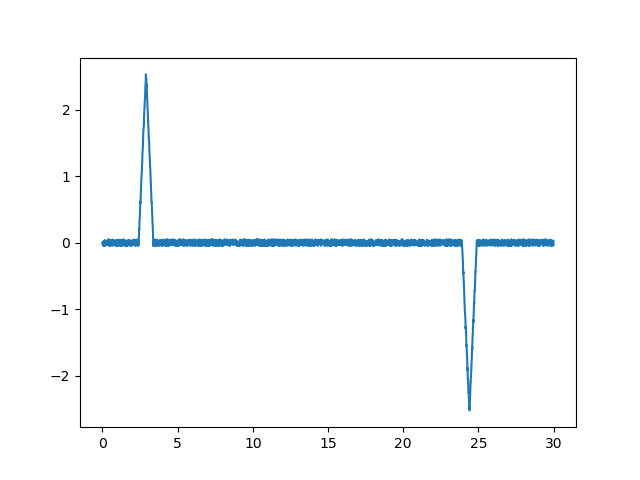
\includegraphics[width=0.5\linewidth]{Code/figure1}
 \caption{Accélération (m.s$^{-2}$) de l'ascenseur au cours du temps (s)}
  \label{fig1}
 \end{center}
\end{figure}

\begin{enumerate}
\item \begin{enumerate}
\item Ouvrir le fichier, traiter les données pour les stocker dans des listes \verb?temps? et \verb?acceleration?. Tracer \verb?acceleration? en fonction de \verb?temps?, cela devrait donner le même tracé que celui de la figure \ref{fig1}.
\begin{solution}~\ \\
\begin{verbatim}
fichier=open('data.csv','r')
contenu=fichier.read()
lignes=contenu.split('\n')
temps=[]
acceleration=[]

for ligne in lignes[1:-1]:
    temps.append(float(ligne.split(";")[0]))
    acceleration.append(float(ligne.split(";")[1]))
    
plt.plot(temps,acceleration)
\end{verbatim}
\end{solution}
\item Soit \verb?f? une liste des valeurs d'une fonction à des instants définis dans une liste \verb?t?. Définir une fonction \verb?integration_num(t,f,f0)? qui renvoie une liste des différentes valeurs de l'intégrale de la fonction à partir de la méthode des rectangles. \verb?f0? est la valeur à l’origine de l'intégrale.
\begin{solution}~\ \\
\begin{verbatim}
def integration_num(t,f,f0):
    fi=[f0]
    for i in range(1,len(f)):
        fi.append(fi[i-1]+f[i]*(t[i]-t[i-1]))
    return fi
\end{verbatim}
\end{solution}
\item Utiliser cette fonction pour déterminer la vitesse puis la position de l'ascenseur au cours du temps sous la forme de listes \verb?vitesse? et \verb?position?. On prendra les conditions initiales nulles ($vitesse(0)=0$ et $position(0)=0$).
\begin{solution}~\ \\
\begin{verbatim}
vitesse=integration_num(temps,acceleration,0)
position=integration_num(temps,vitesse,0)
\end{verbatim}
\end{solution}
\item Tracer \verb?position? en fonction de \verb?temps?.
\begin{solution}~\ \\
\begin{verbatim}
plt.plot(temps,position)
plt.show()
\end{verbatim}
\begin{figure}[!ht]
 \begin{center}
 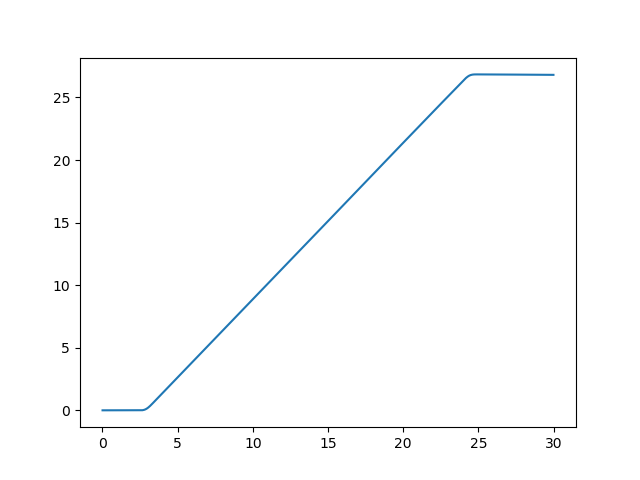
\includegraphics[width=0.5\linewidth]{Code/figure2}
 \caption{Position (m) de l'ascenseur au cours du temps (s)}
  \label{fig2}
 \end{center}
\end{figure}
\end{solution}
\item Un étage mesurant 3 m, afficher le nombre d'étages parcourus.
\begin{solution}~\ \\
\begin{verbatim}
print(position[-1]/3.)
\end{verbatim}
On trouve 9 étages (valeur approchée à cause des erreurs de mesure.)
\end{solution}
\end{enumerate}
\end{enumerate}

\section*{Fabrication d'une fonction à partir d'une liste de coordonnées}

Pour la suite de l'exercice, il est nécessaire que l'accélération soit stockée sous la forme d'une liste de coordonnées afin d'être manipulée et consultée comme une fonction $a(t)$ dont l'entrée serait un instant $t$ et la sortie l'accélération correspondante (l'exemple donné présente le mode d'utilisation de la fonction mais les valeurs ne correspondent pas à ce qui doit être trouvé) :
\begin{verbatim}
print a(10)
>>> 8.999
\end{verbatim}

La réalisation de cette fonction doit se faire en deux étapes:
\begin{itemize}
 \item déterminer à quel index de la liste correspond le temps $t$ donné en entrée,
 \item afficher l'accélération dont l'index est la valeur trouvée précédemment.
\end{itemize}

\begin{enumerate}
\item \begin{enumerate}
\item Proposer une fonction \verb?index_temps(t,data_temps)? qui renvoie l'index du temps juste inférieur à \verb?t? dans la liste \verb?data_temps?.
\begin{solution}~\ \\
\begin{verbatim}
def index_temps(t,data_temps):
        i=0
        while data_temps[i]<t:
                i=i+1
        return i
\end{verbatim}
\end{solution}
\item Proposer une fonction \verb?a(t)? qui utilise la fonction \verb?index_temps? afin de donner l'accélération associée à un instant \verb?t? par la méthode précédente.
\begin{solution}~\ \\
\begin{verbatim}
def a(t):
        return acceleration[index_temps(t,temps)]
\end{verbatim}
\end{solution}
\item En sachant que $\dfrac{d\ v(t)}{dt}=a(t)$, déterminer grâce à la méthode d'Euler la liste \verb?v_list? des coordonnées de la fonction vitesse $v(t)$.
\begin{solution}~\ \\
\begin{verbatim}
def methode_euler(F,y0,t):
        y = [0]*len(t)
        y[0] = y0
        for i in range(len(t)-1):
                y[i+1] = y[i]+(t[i+1]-t[i])*F(t[i])
        return y

v_list=methode_euler(a,0,temps)
\end{verbatim}
\end{solution}
\item Proposer une fonction \verb?v(t)? qui utilise la fonction \verb?index_temps? afin de donner la vitesse associée à un instant \verb?t? par la méthode précédente en utilisant la liste \verb?v_list?.
\begin{solution}~\ \\
\begin{verbatim}
def v(t):
        return v_list[index_temps(t,temps)]
\end{verbatim}
\end{solution}
\item En sachant que $\dfrac{d\ p(t)}{dt}=v(t)$, déterminer grâce à la méthode d'Euler la liste \verb?p_list? des coordonnées de la fonction position $p(t)$.
\begin{solution}~\ \\
\begin{verbatim}
p_list=methode_euler(v,0,temps)
\end{verbatim}
\end{solution}
\item Proposer une fonction \verb?p(t)? qui utilise la fonction \verb?index_temps? afin de donner la position associée à un instant \verb?t? par la méthode précédente en utilisant la liste \verb?p_list?.
\begin{solution}~\ \\
\begin{verbatim}
def p(t):
        return p_list[index_temps(t,temps)]
\end{verbatim}
\end{solution}
\item Tracer les listes \verb?p_list? et \verb?position? en fonction de \verb?temps?. Le résultat vous paraît-il satisfaisant ?
\begin{solution}~\ \\
\begin{verbatim}
plt.plot(temps,position)
plt.plot(temps,p_list)
plt.show()
\end{verbatim}
Le résultat est satisfaisant car les courbes se superposent.
\begin{figure}[!ht]
 \begin{center}
 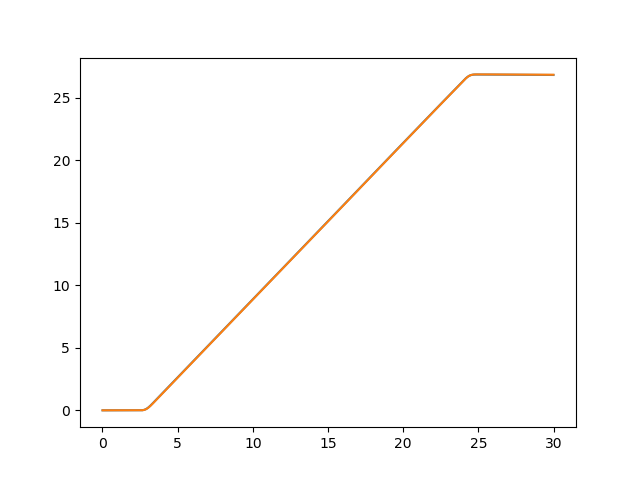
\includegraphics[width=0.5\linewidth]{Code/figure3}
 \caption{Position (m) de l'ascenseur au cours du temps (s) par les deux méthodes}
  \label{fig3}
 \end{center}
\end{figure}
\end{solution}
\end{enumerate}
\item On souhaite rechercher une position particulière. A l'aide de la méthode de Newton, déterminer l'instant \verb?t? à partir duquel l'ascenseur est à 12m du sol (4 étages).
\begin{solution}~\ \\
\begin{verbatim}
def p2(t):
    return p(t)-12.

def methode_Newton(f,df,a,p) :
    x0=a
    while abs(f(x0))>p : # ou abs(e)>p
        x1=x0-f(x0)/df(x0)
        e=x1-x0
        x0=x1
    return x1

print(methode_Newton(p2,v,5,10**(-2)))
\end{verbatim}
\end{solution}        
\end{enumerate}

\end{document}
